\chapter{Hardware}
\section{Schéma zapojenia}
Schéma zapojenia je pomerne jednoduchá obr.\ref{OBRAZOK 1.1}. Jej najdôležitejšiu časť tvorí operačný zosilňovač MCP602 obr.\ref{OBRAZOK 1.2}. Operačný zosilňovač je jednosmerne viazaný elektronický zosilňovač napätia s vysokým ziskom s diferenciálnym vstupom a zvyčajne s jednosmerným výstupom. V tejto konfigurácii optický zosilňovač vytvára výstupný potenciál (vzhľadom na zem obvodu), ktorý je zvyčajne 100 000-krát väčší ako rozdiel potenciálov medzi jeho vstupnými svorkami.

\begin{figure}[!tbh]
\centering

\includegraphics[width=\textwidth]{obr/schema.png}
\caption{schéma zapojenia.}\label{OBRAZOK 1.1}
\end{figure}

Na tento zosilňovač máme pripojený elektrický kondenzátorový mikrofón obr.\ref{OBRAZOK 1.3}. Skladá sa z dvoch platní, jednej pevnej a druhej pohyblivej. Vibrácie vzduchu sa transformujú na posun pohyblivej membrány, ktorá vytvára zmenu elektrického potenciálu. Túto zmenu zachytáva  snímač, ktorý následne vysiela elektrický signál. Elektrický signál sa zosilní a následne je spracovaný v arduine.

\begin{figure}[!tbh]
\centering
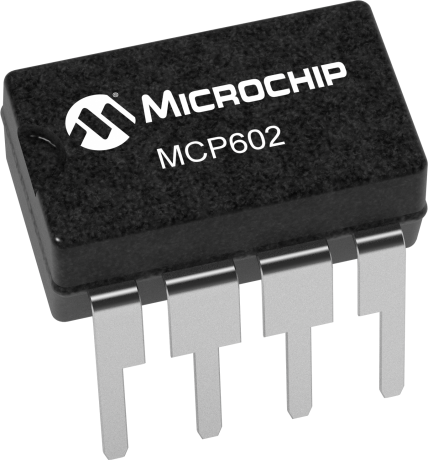
\includegraphics[width=8cm]{obr/mcp.png}
\caption{{operačný zosilňovač MCP602.\cite{mcp}}}\label{OBRAZOK 1.2}
\end{figure}

\begin{figure}[!tbh]
\centering
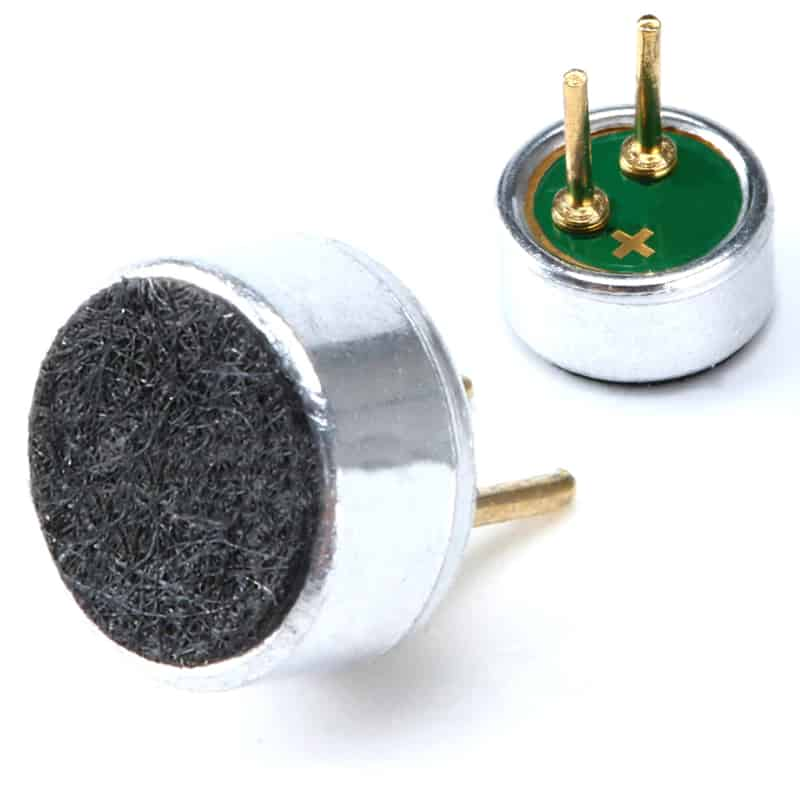
\includegraphics[width=7cm]{obr/mike.jpg}
\caption{{elektrický kondenzátorový mikrofón.\cite{mike}}}\label{OBRAZOK 1.3}
\end{figure}

Ďalšou kritickou časťou systému je infračervená LED dióda, pomocou ktorej posielame signály potrebné na ovládanie televízora. Je dôležité podotknúť že nie všetky televízory resp. ovládače, fungujú na princípe infračervenej LED diódy, avšak v dnešnej dobe pracuje na tomto princípe väčšina zariadení. LED dióda vysiela špeciálne príkazy pomocou modulácie dĺžok medzier medzi vyslanými signálmi ktoré následne zachytáva a spracováva televízor.

Následne sa na doske nachádzajú aj 2 potenciometre ktoré slúžia na nastavovanie hodnôt potrebných pre správne fungovanie API a 2 LED diódy, jedna zelená, druhá červená, ktoré slúžia len na vizuálnu kontrolu fungovania systému keďže infračervené lúče vysielané IR LED diódou sú pre naše oči neviditeľné.

Na schéme môžeme takisto vidieť IR snímač VS1838B ktorý sme chceli využiť na zapisovanie signálov na zvyšovanie a znižovanie hlasitosti. Na spustenie tejto funkcie slúži tlačidlo s názvom BUTTON ktoré je tiež viditeľné na schéme. Žiaľ, túto funkciu sa nám nepodarilo úspešne implementovať do nášho kódu. Problémom pri spolupráci na projekte bol lockdown a nemožnosť spoločnej práce v reálnom svete ale iba pomocou online komunikácie. Práca s hardwarom tak bola náročnejšia a testovanie kódu, ktorý sme napísali, bolo obmedzené.

Hlavným nedostatkom tohto kódu bolo správne zapísanie získaných hodnôt do funkcie IRsenderu. Kód sme úspešne detegovali a vedeli ho uložiť do pamäte EEPROM, no následné zapísanie uloženého kódu a jeho poslanie nefungovalo ani po mnohých iteráciách. Kód bol teda na \verb|99%| funkčný, ale jeho najdôležitejšia časť, posielanie signálov, nám nechcela fungovať. V situácii kedy by bolo na projekt viacej času, túto funkciu by sme radi implementovali do ovládača hlasitosti.





